% \section{Introduction}
% In this assignment we had to parallelize the Conjugate Gradient method using GPUs and the CUDA libraries. In order to do
% this I first implemented all the cBLAS functions used as CUDA kernels. These implementations can be found in the
% \lstinline[language=C]|cuda_ops.cu| file. These are almost a direct replacement to the cBLAS functions, however, minor
% differences do exist. The doc strings for each function can be found in the \lstinline[language=C]|cuda_ops.hh| file,
% which document their usage. The \lstinline[language=C]|config.hh| file can be used to turn on different options before
% compiling the file, such as DEBUG mode. The \lstinline[language=C]|cg_solver| binary accepts 2 arguments, the first
% being the path to the mtx matrix file and the second being the number of threads to assign to each block. When running
% on Izar this can be set to a maximum of 1024 threads per block.

\section{Scaling Experiments}
To test the performance of my code I ran thread scaling experiments on Izar. To do this I changed the maximum number of
threads per block (second argument to the cg\_solver binary) and ran the program 5 times to compute an average.
The threads were scaled in a logarithmic fashion using base 2. The results can be found in the graph below.

\begin{figure}[h!]
    \centering
    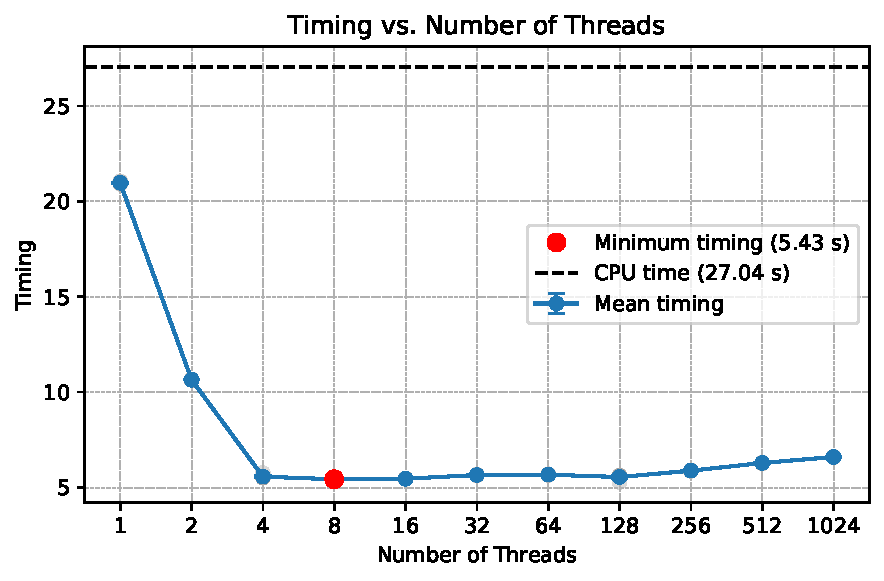
\includegraphics[width=0.75\textwidth]{plots/timing_vs_threads.pdf}
    \caption{Results of thread scaling experiments}
\end{figure}

\FloatBarrier

Overall the GPU code is faster than the CPU code even when we only assign one thread to each block. Also, as expected
the runtime decreases initially as more threads are added reaching a minimum at 8 threads per block. This makes sense
are the algorithm is running more operations in parallel so the runtime is expected to decrease. From 4-64 threads per
block, the runtime stays roughly constant only varying by a 0.2 seconds, this that perhaps the algorithm is not
compute-bound but rather bound by memory transfers speeds. This is further confirmed by the fact that adding more than
64 threads per block actually increases the runtime, until at 1024 threads per block the runtime is slower than with 4
threads per block. To investigate this bottleneck further I profiled the 1024 threads per block run with nvprof.
{
\small
\begin{lstlisting}[language=C]
template <typename T>
__global__ void cu_dgemv(T* c, const  T* A, const T* x, const T alpha, const T beta, size_t m, size_t n){
    size_t matrix_row = blockIdx.x * blockDim.x + threadIdx.x;
    if (matrix_row < m) {
        T sum = 0;
        for (size_t i = 0; i < n; i++) {
            sum += A[matrix_row * n + i] * x[i];
        }
        c[matrix_row] = alpha * sum + beta * c[matrix_row];
    }
} 
\end{lstlisting}
}
The profiling showed that 96.96\% of the runtime was spent on the \lstinline[language=C]|cu_dgemv| kernel, which computes
a matrix vector product. Since the operations themselves are simple, the long runtime is likely due to inefficient
memory access when retrieving the value of \lstinline[language=C]|A[matrix_row * n + i]|. Since these values are not
sequential in memory the streaming multiprocessor frequently has to access global GPU memory rather due to cache misses
in its local memory. One way to improve this would be to use shared memory to preload the relevant values of A and x
before starting the computations. While this would introduce some initial overhead, it would greatly speed up
computation since the streaming multiprocessor would be able to fetch values from shared memory which is much faster
than global memory. Loop unrolling was also tested to see if performance would improve, however no significant gains
were noticed and hence it was removed. 